% !TEX root = ../thesis-example.tex
%
\chapter{Metodologia}
\label{Metodologia}

En este capitulo se presenta el metodo y algoritmos desarrollados para calculo de la entropia en mercados financieros.
La metodologia presentada tiene como objetivo ayudar a detectar si un mercado es \textit{estable} en el tiempo a partir de la entropia calculada.
Adicionalmente, el metodo propuesto puede ser utilizado para detectar momentos (fechas) en los que la entropia es minima. 
Esto se traduce como un intervalo de tiempo en el que el precio no cambia significativamente.


Descripcion de metodo aplicado para entropia  ver diagrama \ref{diagramaentropia1}.

\begin{figure}[h]
	\centering
	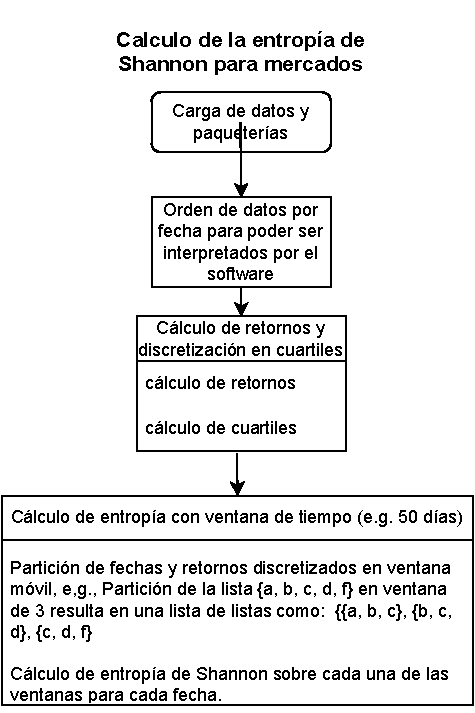
\includegraphics[width=0.7\linewidth]{figures/diagrama_entropia1}
	\caption{Diagrama del algoritmo utilizado para el c\'alculo de entrop\'ia de Shanon en mercados financieros.}
	\label{diagramaentropia1}
\end{figure}


\section{Algoritmo para el calculo de entropia}

La metodologia implementada para el calculo de la entropia asi como el procesamiento de datos se presenta en el diagrama \ref{diagramaentropia1}.
En este diagrama se identifican cuatro etapas principales:

\begin{itemize}
	\item Carga de datos
	\item Pre-procesamiento de datos
	\item Calculo de retornos y cuartiles
	\item Calculo de entropia
\end{itemize}

\subsection{Procesamiento de datos de precios de mercados}

Los precios de los mercados utilizados en esta Tesis fueron obtenidos del portal Yahoo Finance. 
Cabe mencionar que los precios son registrados cada 24h excepto los dias sabado y domingo.
Se descargaron las datos de precios entre DD/MM/YYYY y DD/MM/YYYY de los mercados AAA, BBB, CCC, y DDD.

Un ejemplo de la base de datos de precios descargada se presenta en la tabla \ref{ejemplo_data}.
Las columnas de la base de datos corresponden a la fecha en la que se realizo el registro de precio respectivo.
Las bases de datos de cada uno de los mercados fueron depuradas y ordenadas. Esta depuracion corresponde a identificar y eliminar las fechas en las que no hay precio registrado. De este modo se evitan errores de calculo.

\begin{center}
\begin{tabular}{|c|c|}
	\hline 
	Fecha & precio \\ 
	\hline 
	DD/MM/YYYY & $$$$ \\ 
	\hline 
	DD/MM/YYYY & $$$$ \\ 
	\hline 
	DD/MM/YYYY & $$$$ \\ 
	\hline 
\end{tabular} 
	\label{ejemplo_data}
\end{center}

\subsection{Calculo de retornos de precios de mercados}

Luego que se han cargado los datos, y se han ordenado es necesario calcular los retornos de los precios. 
%y ello conlleva a que no va a haber una media central en los datos. 
Los retornos permiten analizar fácilmente la tasa de cambio en el tiempo.
En esta Tesis se eligio trabajar con los retornos de los precios y no con los precios directamente debido a las propiedades de los retornos presentadas en la subseccion \ref{retornos}.
Aunque los retornos son una mejor representación de los precios, aún presentan picos que sobresalen de la media. 
%La estandarización permite destacar los retornos que realmente son relevantes. 
%%%-----NO SE APLICO ESTANDARIZACION NO ?????
%Ya que cada retorno ha sido estandarizado con su respectiva fecha,  
Posteriormente se procede a discretizar los retornos mediante un proceso que divide en cuatro intervalos a los retornos. 
Esto se hace mediante el calculo de los cuartiles de los retornos. 
A cada cuartil se le asigna una etiqueta lo que permite discretizarlos . 
En otras palabras, los intervalos van a permitir etiquetar del 1 al 4 a cada retorno. 

\begin{center}
	\begin{tabular}{|c|c|c|}
		\hline 
		Fecha & retorno & cuartil \\ 
		\hline 
		DD/MM/YYYY & $$$$ & 1\\ 
		\hline 
		DD/MM/YYYY & $$$$ & 2\\ 
		\hline 
		DD/MM/YYYY & $$$$ & 4\\ 
		\hline 
	\end{tabular} 
	\label{ejemplo_data-returns}
\end{center}

\subsection{Calculo de la entropia}

La ecuación de la entropía requiere conocer la probabilidad de los elementos del sistema, 
con los intervalos dados por los cuartiles y la discretización de los retornos se obtiene todo lo necesario para calcular la entropía, sin embargo, no se calcula la entropía de todo el conjunto de datos, se hace por subconjuntos de datos agrupados en listas de 50 elementos, o cualquier número dado por el usuario.

El resultado de la entropia es dado en valores y fechas para cada subconjunto de días.




\subsection{Entropía utlizando medias moviles}

Se aplica el mismo metodo mencionado arriba, adicionalmente en la etapa en que se estandarizan los retornos de los precios con su respectiva fecha ( ver Figura \ref{entropiamav}). La ventana puede ser elegida por el usuario. Se aplica una entrada de por lo menos 50 días ya que un número menor no suavizaría la curva de manera que no se podría apreciar tendencias en el comportamiento de la curva.





\begin{figure}
	\centering
	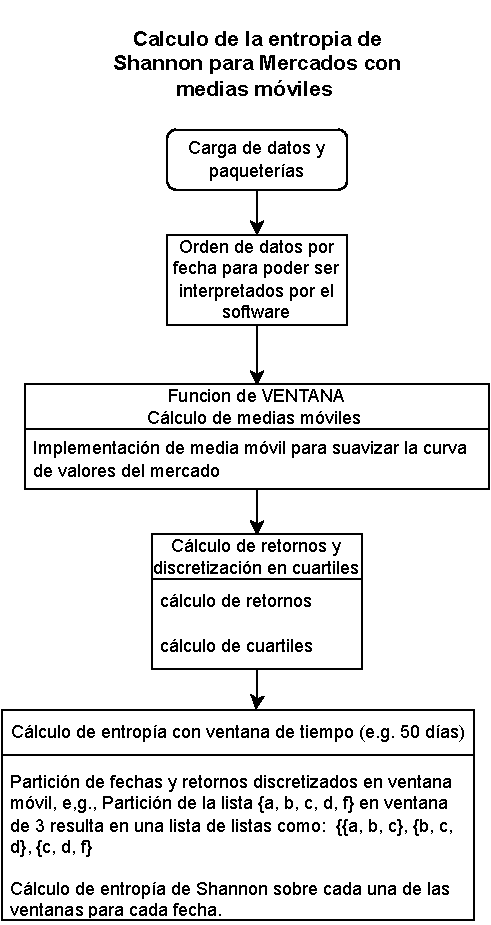
\includegraphics[width=0.7\linewidth]{figures/entropiaMAV}
	\caption{Diagrama del algoritmo utilizado para el c\'alculo de entrop\'ia de Shanon en mercados financieros con medias m\'oviles.}
	\label{entropiamav}
\end{figure}

La simulación de un mercado eficiente requiere cargar datos debido a que se simula un caminante aleatorio a partir de una distribución gaussiana con una media y desviación estándar obtenidas del análisis de los retornos (no estandarizados) de los precios reales. 

Del paso anterior se obtienen retornos simulados, mismos que deben estandarizarse y asignarles su fecha.

A partir de este punto hay dos situaciones que se pueden apreciar en el diagrama \ref{simulacion}, la primera es que a dichos retornos simulados se les aplica el proceso para el cálculo de entropía de la figura \ref{diagramaentropia1}, y la segunda es que se aplica el proceso de medias móviles como se presenta en \ref{entropiamav}.


Se destacan valores mínimos de entropía gracias a la manera en que se presentan los resultados, con ello comparar el comportamiento de la entropía del mercado eficiente y del mercado real con fechas, con o sin media móvil requiere únicamente del cálculo de un umbral que diferencie los valores de entropía que se comportan de manera gaussiana  de los que no.

Mediante la definición de un umbral que permite seleccionar con un intervalo de confianza de 95 porciento los valores de entropía mínima en los mercados. 

\begin{figure}
	\centering
	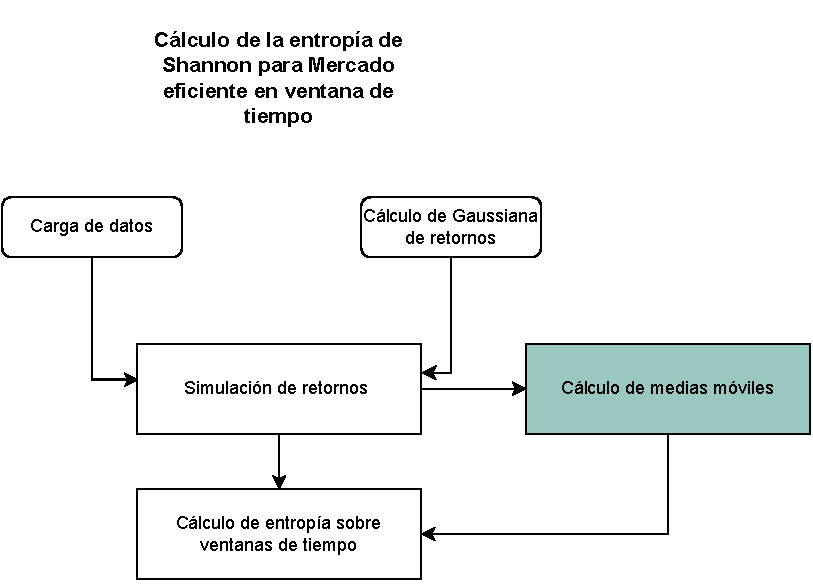
\includegraphics[width=0.9\linewidth]{figures/simulacion}
	\caption{Diagrama del algoritmo de calculo de entropia para la simulacion de mercado eficiente. }
	\label{simulacion}
\end{figure}

Reglas de cuartiles
\begin{center}
	\begin{tabular}{ |r | l | c| }
		 \hline
		Cuartiles & Regla & Valor de retorno discretizado \\ \hline
		Primer cuartil & $(-\infty , Q_2)$ & 1 \\
		Segundo cuartil & $[Q_2 , Q_3)$   & 2\\ 
		Tercer cuartil &  $[Q_3 , Q_4)$   & 3 \\
		Cuarto cuartil & $[Q_4 , \infty)$ &4\\ 
		 \hline
	\end{tabular}
\end{center}



Finalmente, se aplica una prueba estadística de distribuciones a los valores con mínima entropía, tanto de aquellos que fueron tratados con un filtro de media movil como aquellos que no. 


\textbf{¿Por qué se utiliza la función Quantile para obtener el intervalo de confianza?}



Recordemos que de la ecuación de la entropía de Shannon, se realiza la suma de la probabilidad del estado, multiplicado por la probabilidad del estado. Gracias a que se trabajan con probabilidades es posible graficar un histograma de las entropías, y además se puede estudiar la entropía mediante cuantiles de manera análoga con los retornos de los precios.

Calcular el intervalo de confianza para la distribución de estas entropías sale de este trabajo de tesis, ya que no se asemeja ni a una distribución normal ni a una distribución de Student, ello implicaría tener que realizar interpolaciones entre los cuantiles obtenidos tal como se muestra en el articulo A Method for Confidence Intervals of High Quantiles de Mei Ling Huang, y Xiang Raney-Yan publicado en 2021. 
%file:///D:/dark_/descarga_chrome/entropy-23-00070-v3.pdf

Por lo anterior, se propone utilizar como umbral para hallar los valores mínimos de entropía el valor del percentil 95 en vez de un íntervalo de confianza. Entre el año 2000 y 2005, se aprecia un valor mínimo en el precio, mismo que tiene impacto al estudiar la entropía.


Entonces, al realizar un gráfico que muestra la distribución de la entropía, y dado que la entropía es obtenida a partir de probabilidades, es fácil obtener cualquier cuantil (percentil 95 en el caso del intervalo de confianza), además que dicho percentil permite diferenciar aquellos valores de la entropía que son ruido de aquellos que no. 

